\thispagestyle{empty}
\begin{center}
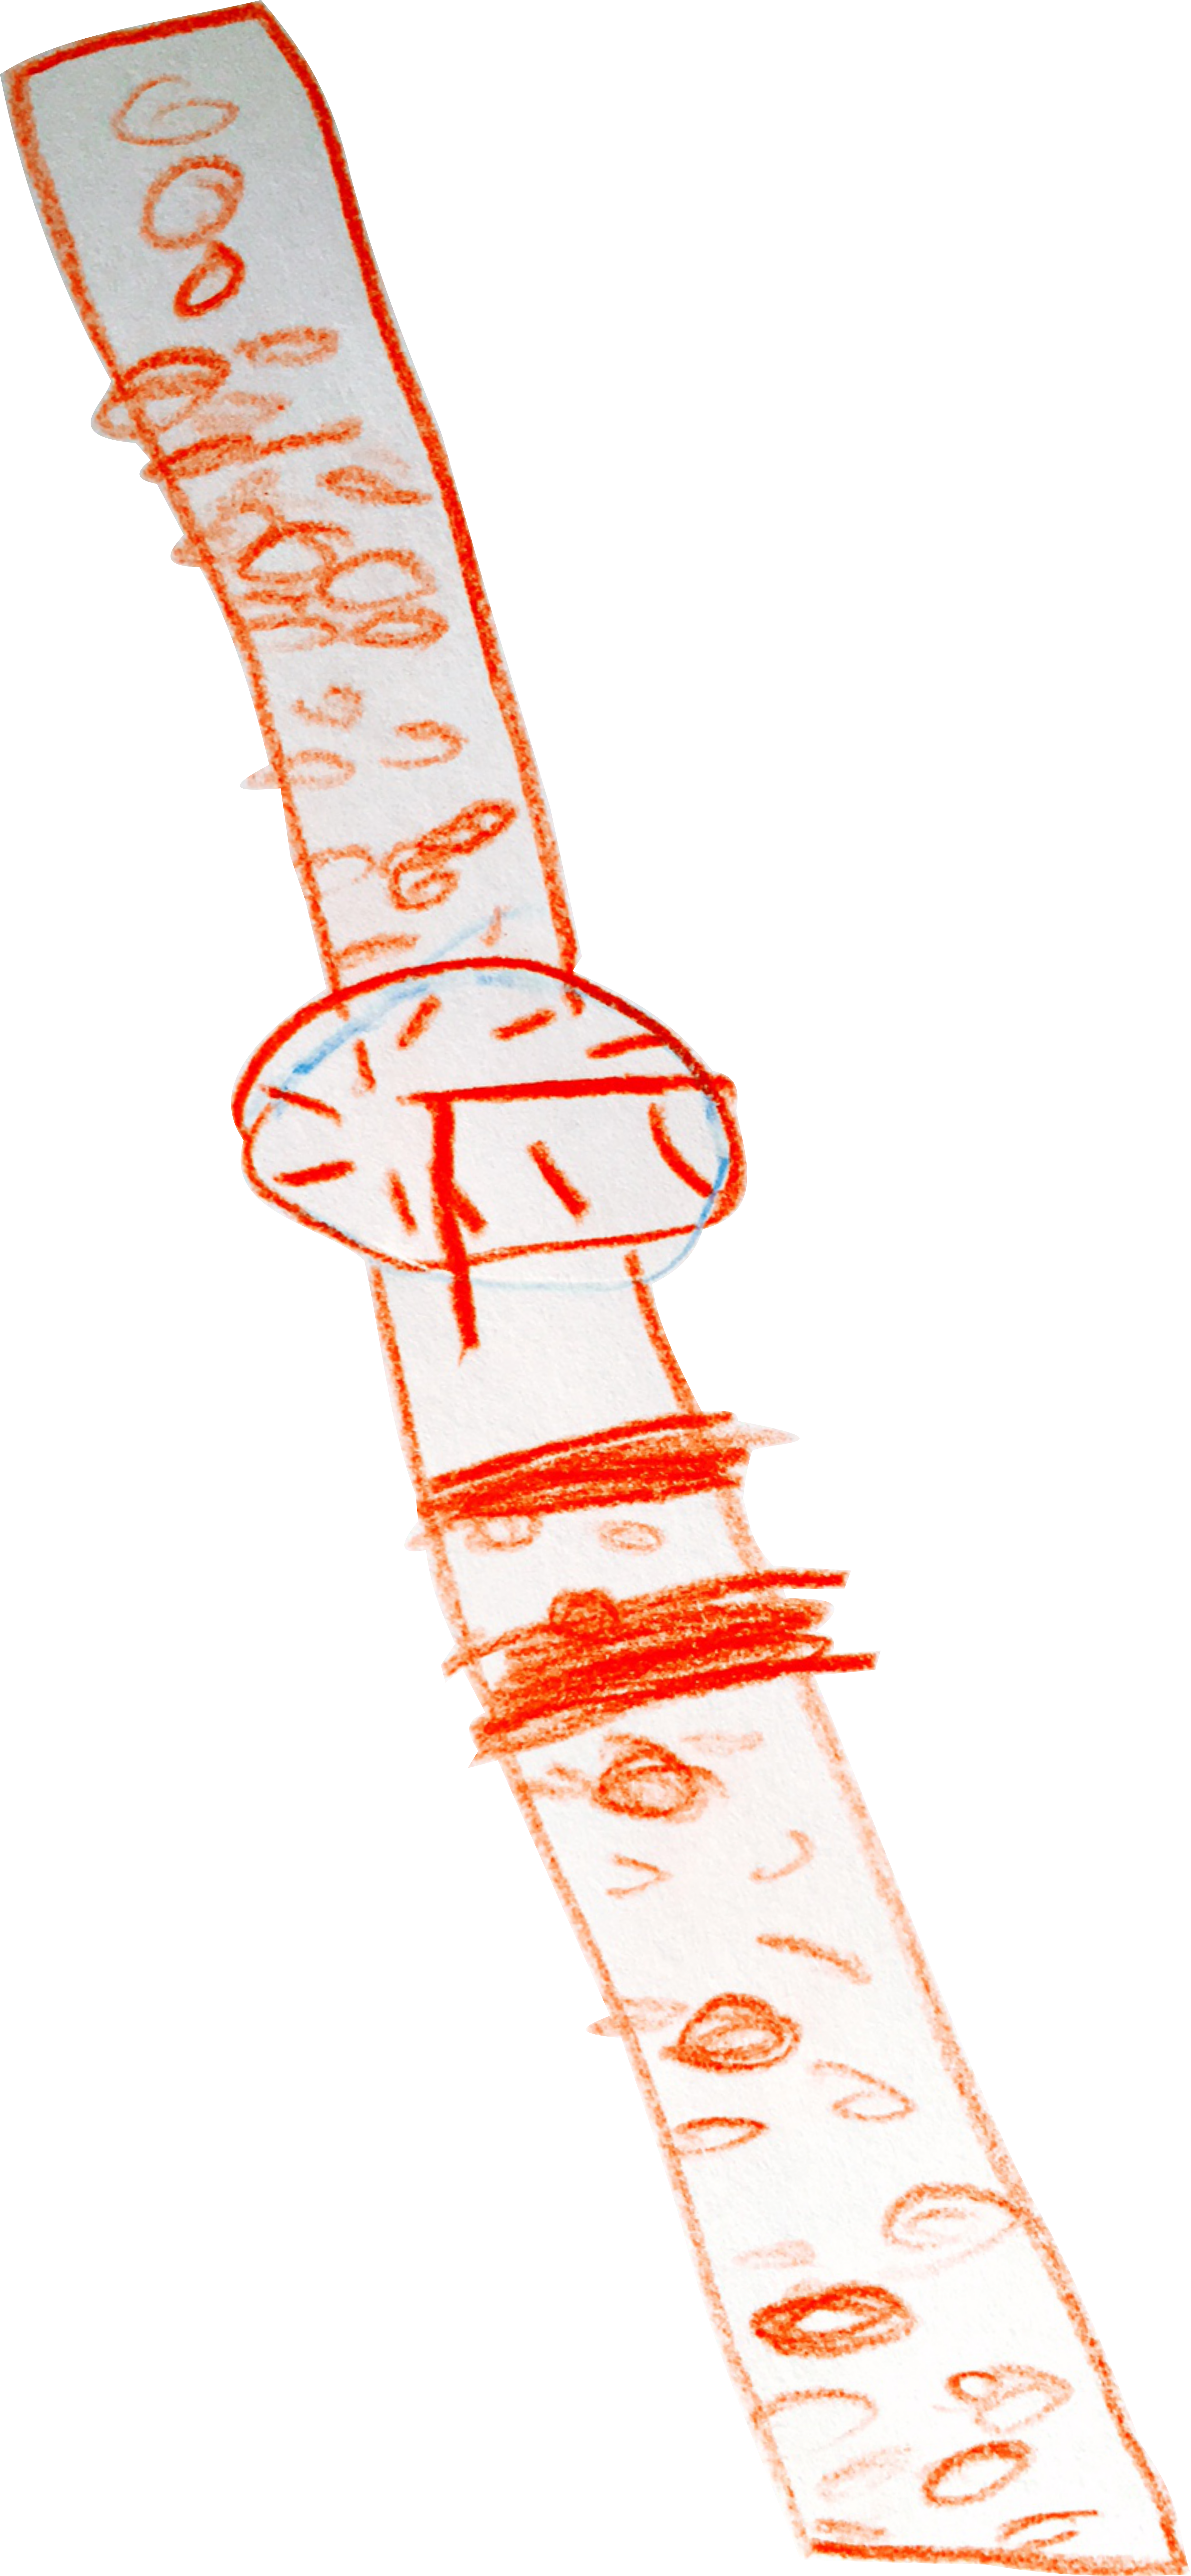
\includegraphics[height=.8\textheight]{./bilder/160120_uhr.png}
\end{center}
\vskip 2cm
{\Huge\color{farbe}\hfill{\tt{}}}
\addcontentsline{toc}{chapter}{}
\newpage
%%%%%%%%%%%%%%%%%%%%%%%%%%%%%%%%%%%%%%%%%%%%%%%%%%%%%%%%%%%%%%%%%%%%%%%%%%%%%%%
\lettrine[lines=2, lhang=.2, loversize=.25, lraise=0.05, findent=0.1em,
nindent=0em]{A}{}
Dem Grüffelo sitzt vor seiner Höhle. Sein Magen knurrt so laut, dass die Blätter in den Ästen wackeln. Aber an der Hunger ist gar nicht einmal das Schlimmst. Eine Maus hat ihn ausgetrickst. Ihn, den grossen und gefährlichen Grüffelo. Ihn, vor dem alle im Wald Angst haben. 

Na ja, vermutlichen Angst hatten. Nachdem die Maus ihm weiss gemacht hatte, dass sie so gefährlich und grauenhaft ist, dass sich sogar die Eule, die Schlange und der Fuchs vor ihr fürchten, hatte er schnell Reissaus genommen. Ein Reh hatte ihn gesehen, wie er zu seiner Höhle gerannt ist. Und er, der mächtige Grüffelo hatte ihm im Vorbeirennen zugerufen, es solle sich in Acht nehmen, die Maus sei in diese Richtung unterwegs. 

Das Reh hatte sofort begriffen, was passiert war. Die kleine Maus hatte alle gefährlichen Tiere hereingelegt. Die Schadenfreude war riesig und noch schneller als er, der Grüffelo in seiner Höhle angekommen war, hatte sich die Nachricht im ganzen Wald verbreitet. 

Und ein Grüffelo ist kein Grüffelo mehr, wenn ihn alle auslachen. Die gifitge Warze auf seiner Nase juckte gewaltig bei bei dem Gedanken. Drei Tage lang traute sich der Grüffelo nicht mehr aus seiner Höhle. Ganz nach hinten hatte er sich verzogen, da wo es kalt und nass war und Pilze wuchsen.

Vor lauter Hunger ass er einfach so einen Pilz. Jetzt ist ja auch alles egal, dachte er sich dabei. Aber wie gross war seine Überraschung, wie gut der Pilz schmeckte! Gar nicht so grün und nach vielen Vitaminen wie die Pfalnzen und Beeren, die er so verachtete. Und Tieren musste er auch nicht hinterher jagen, kein Fell, dass man erst abbekommen musste. Und lecker. So ein bisschen wie das Essen, das sein Vater früher immer für ihn gesammelt hatte, als er noch ein kleiner Grüffelo gewesen war. Als seine Klauen noch nicht riesig und die Kniee nicht knotig waren. 

Damals hatte er auch noch viele Freunde hier im Wald. Den Biber zum Beispiel. Aber als er grösser geworden war musste er von zu Hause ausziehen. So ist das bei Grüffelos. Und dann musste er sich einen eigenen Wald suchen. Und da war er jetzt. Von Anfang an gefürchtet, was auch normal ist für Grüffelos. So einen Freund, wie der Biber wäre jetzt prima. Der wüsste was tun. 



\vfill
